
\documentclass[oribib1]{llncs}


%\usepackage{fullpage}
%\documentclass[envcountsame,envcountsect,orivec]{llncs}
\usepackage{amssymb}
\usepackage[latin1]{inputenc}
\usepackage{graphicx}
\usepackage{float}
\usepackage{epstopdf}
\usepackage{makeidx}
\usepackage{bm}
\usepackage{algorithmic}
\usepackage{authblk}
\makeindex
 \usepackage{amsmath} %\usepackage{amstext}
%\usepackage{ntheorem}
\usepackage{hyperref} % NOTE: this may cause you to have to hit compile a couple times initially.
\usepackage{xargs}
\usepackage{tikz}
\usetikzlibrary{matrix}
\usepackage{times}

%\usepackage[margin=2cm]{geometry} %liberal but still acceptable margins
%\usepackage{pslatex} %changes the font to standard ps fonts - saves
%non-negligible space

%\newtheorem{theorem}{Theorem}
%\newtheorem{definition}{Definition}
%\newtheorem{lemma}{Lemma}



%\newenvironment{proof}{\noindent {\bf Proof:} \hspace{.4em}}
%                      {\hspace{\fill}{$\blacksquare$} \smallskip}

%\newenvironment{proofL}{\hspace{.4em}}
%                      {\hspace{\fill}{$\blacksquare$} \smallskip}




%\newtheorem{theorem}{Theorem}[section]
\newtheorem{fact}[theorem]{Fact}
%\newtheorem{claim}[theorem]{Claim}
%\newtheorem{lemma}[theorem]{Lemma}
%\newtheorem{proposition}[theorem]{Proposition}
%\newtheorem{corollary}[theorem]{Corollary}
\newtheorem{obs}[theorem]{Observation}
%\newtheorem{definition}[theorem]{Definition}


\newtheorem{open}{Open Problem}

\newcommand{\troot}{t_{root}}
\newcommand{\troots}{{t_{root}}^*}
\newcommand{\trootss}{{t_{root}}^{**}}
\newcommand{\tbss}{{t_b}^{**}}
\newcommand{\tbs}{{t_b}^{*}}
\newcommand{\trootsFirst}{{t_{root}}^{*First}}
\newcommand{\trootsFinal}{{t_{root}}^{*Final}}
\newcommand{\tbsFirst}{{t_b}^{*First}}
\newcommand{\tmin}{t_{min}}
\newcommand{\tbith}{t_b[{P_i}]}
\newcommand{\tbtwo}{t_b[{P_2}]}
\newcommand{\tblast}{t_b[{P_1}]}
\newcommand{\ra}{\rightarrow}




\begin{document}

\title{Tight Lower Bounds for the Fractional Pebble Game}
\author{Frank Vanderzwet \and
Stephen Cook \and
Toniann Pitassi}
\institute{University of Toronto}

\maketitle
\begin{abstract}
Fractional pebbling is a generalization of black-white pebbling
introduced recently.  Here we solve an open problem by proving a
tight lower bound on the pebble weight required to fractionally
pebble a balanced $d$-ary tree of height $h$.  This bound has a
close connection with the nondeterministic space complexity
of the tree evaluation problem.
\end{abstract}

%\newpage

%\setcounter{section}{0}

\section{Introduction} 

\subsection{Motivation}

The black pebble game was introduced by Paterson and Hewitt \cite{ph:comsc}
to compare the power of programming languages.
Motivated by the problem of separating the complexity classes
{\bf P} (polynomial time) from {\bf NL} (nondeterministic logarithmic
space), it was generalized to the black-white pebble game by Cook and Sethi
\cite{cs:pfromnl} to help in the proof of a super-logarithmic
nondeterministic space lower bound for solving a specific problem in
{\bf P} (Path Systems) on a restricted computation model.   Recently
in \cite{c:pebjournal} it was further generalized to the fractional
pebble game in order study the space complexity of the Tree
Evaluation Problem (TEP), another candidate for separating {\bf P}
and {\bf NL}.

The input to the TEP is a rooted, balanced $d$-ary tree of height $h$
(denoted $T^h_d$),
whose internal nodes are labeled with $d$-ary functions
on $[k]=\{1,\ldots,k\}$, and whose leaves are labeled with elements
of $[k]$.  Each node obtains a value in $[k]$ equal to its $d$-ary
function applied to the values of its $d$ children.  The output is the
value of the root.  In \cite{c:pebjournal} the space complexity of
TEP is studied by measuring the number of states required by $k$-way
branching programs to solve TEP.  There it is shown that the
optimal way of black pebbling the binary tree of height $h$ (which
requires $h$ pebbles) yields a deterministic $k$-way branching
program ($k$-BP) with $\Theta(k^h)$ states, and no $k$-BP with fewer
states solving this problem is known.   A proof of a lower bound on
the number of states required, even if the lower bound was a much smaller
function $k^{r(h)}$, where $r(h)$ is any unbounded function, would
separate {\bf L} from {\bf P}.

In \cite{c:pebjournal} a simple semantic restriction called {\em thrifty}
on $k$-BPs solving TEP was introduced and it was shown that the
$k$-BPs mentioned above (coming from black pebbling) for solving TEP
are thrifty, and in fact their state bound of $\Theta(k^h)$ is the
smallest possible among all thrifty $k$-BPs solving TEP.
(A $k$-BP solving TEP is {\em thrifty} if for every computation
on a labeled input tree, for every query to the function
$f_v(x_1,\ldots,x_k)$ labelling a node $v$, the values of the
arguments $x_1,\ldots,x_k$ for the query must be the actual values of
the children of $v$.)

In \cite{c:pebjournal} nondeterministic $k$-BPs solving the Boolean
TEP problem (BTEP) are also studied, where BTEP has the same input
as TEP, but the problem is
to determine whether the root has value 1.  There the following
result is proved by implementing the algorithm suggested by fractionally 
pebbling the tree $T^h_d$.
\begin{proposition}\label{p:nonDthriftyUP}
There is a nondeterministic thrifty $k$-BP with
$\Theta(k^{p_{frac}(h,d)})$ states which solves BTEP, where $p_{frac}(h,d)$ is
the pebble weight required to fractionally pebble $T^h_d$.
\end{proposition}
In fact no nondeterministic $k$-BP (thrifty or not)
with fewer than $\Theta(k^{p_{frac}(h,d)})$ states solving BTEP is known. 
Similar to the deterministic case, a proof of even a much
weaker lower bound on the number of states required would separate
{\bf NL} from {\bf P}.

In the present paper we establish exact values for $p_{frac}(h,d)$ for
all $h,d \ge 2$.  Although approximate values were known previously
(see Proposition \ref{p:fracvalue}), the complicated proof depends on
Klawe's \cite{k:bwpyr} elaborate lower bound proof for black-white pebbling
of DAGs.  We present a direct proof by induction on the height of the tree.

A major motivation for giving our direct proof for tight lower bounds on
fractional pebbling numbers is the hope of using ideas in the proof to
establish that the bound given in Proposition \ref{p:nonDthriftyUP}
for nondeterministic thrifty BPs solving BTEP is tight.  Such a tight
lower bound has been proved for the deterministic case
(see Theorem 33 in \cite{c:pebjournal}), and the proof proceeds by associating
a black pebbling with every computation of a deterministic thrifty BP
that solves TEP, and showing that if the pebbling uses $p$ pebbles then
the BP must have at least $k^p$ states.   The hope (not yet realized)
is to associate a fractional pebbling with every accepting
computation of a nondeterministic thrifty BP solving BTEP so as to get an
analogous result. 



\subsection{Pebbling}

Here we are interested in the pebble game on rooted $d$-ary trees,
although there is a natural generalization to rooted DAGs.
We define three versions.
The first is the simple `black pebble' game:  A black
pebble can be placed on any leaf, and in general
if all children of a node $i$ have pebbles, then one of the
pebbles on the children can be slid to $i$ (this is a
``black sliding move')'.  Any black pebble can be removed
at any time.  The goal is to pebble the root, using as few
pebbles as possible.

The second version is (whole) black-white pebbling
with the restriction that we do not allow
``white sliding moves''.  Thus if node $i$ has a white
pebble and each child of $i$ has a pebble (either black or white)
then the white pebble can be removed.  (A white sliding move
would apply if one of the children had no pebble, and the
white pebble on $i$ was slid to the empty child.  We do not
allow this, because there is no corresponding move in a $k$-way branching
program solving TEP.)  A white pebble can be placed on any node at
any time.  The goal is to start and end with no pebbles,
and to have a pebble on the root at some time.

The third version is fractional pebbling,
which generalizes whole black-white pebbling by allowing the
black and white pebble weight of a node to be any real number
between 0 and 1.  However the total pebble weight of each
child of a node $i$ must be 1 before the black weight of $i$
is increased or the white weight of $i$ is decreased.

Figure \ref{f:bin_h3_fract_ub} illustrates
an optimal fractional pebbling with pebble weight 2.5 of the binary tree of
height three.

\begin{figure}
\vspace*{-1.5cm}
\hspace*{1.5cm}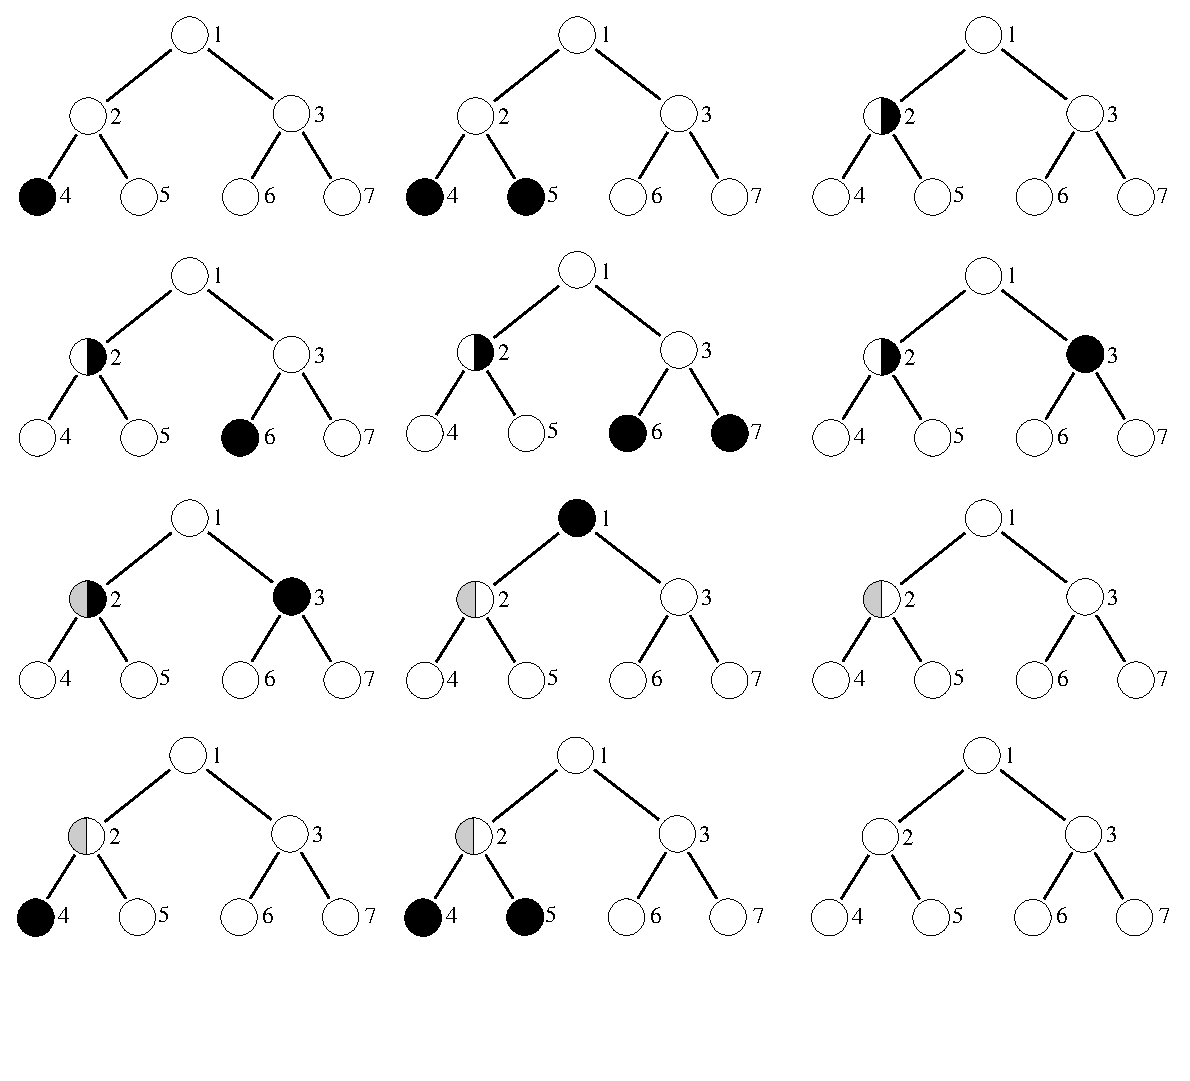
\includegraphics[scale=0.70]{bin_h3_fract_ub_full.eps}
\vspace*{-1.5cm}
\caption{An optimal fractional pebbling sequence for the height 3 tree
using 2.5 pebbles, all configurations included (except the empty starting config).
The grey half circle
means the \emph{white} weight of that node is $.5$, whereas unshaded
area means absence of pebble weight. So for example in the seventh
configuration, node 2 has black weight .5 and white weight .5, node 3
has black weight 1, and the remaining nodes all have black and white
weight 0. }
\label{f:bin_h3_fract_ub}
\end{figure}

The motivation for choosing these definitions is that we want
pebbling algorithms for trees to closely correspond to $k$-way
branching program algorithms for solving TEP.  The idea is that
a whole black pebble on a node means that the corresponding branching
program state `knows' the value of the node, and a whole white pebble
(applicable to nondeterministic BPs)
means that that state has a specific conjecture for the value of the
node (which must later be verified).  A fractional pebble $w$,
$0\le w\le 1$, on a node means that the current state knows or conjectures
a fraction $w$ of the $\log k$ bits needed to specify the value of the
node.

The {\em pebble weight} of a pebble configuration is the sum
over all nodes $i$ of the pebble weight of $i$.
The {\em pebble weight} of a pebbling of a tree is the maximum,
over all configurations $c$ of the pebbling, of the pebble weight of $c$.

Recall that $T^h_d$ is the balanced $d$-ary tree of height $h$
(i.e. $h$ levels).  

\begin{definition}\label{d_p-def}
$p_{black}(h,d)$ (resp. $p_{bw}(h,d)$, $p_{frac}(h,d)$) is the minimum
pebble weight over all black (resp. black-white, fractional) pebblings
of $T^h_d$.
\end{definition}

The exact values of $p_{black}$, and for many cases of $p_{bw}$, have been
known for some time \cite{nord:survey2,c:pebjournal}.
%and approximate values for
%$p_{frac}$ were first proved in \cite{c:pebjournal}.

\begin{proposition}\label{p:pebble_value}
\begin{eqnarray}\label{e:black}
  & p_{black}(h,d) = (d-1)h-d+2  \\
  & \mbox{$p_{bw}(h,d) = \lceil(d-1)h/2\rceil +1$ for $d=2$ and $d$ odd}
\end{eqnarray}
\end{proposition}

From \cite{c:pebjournal} we have the following bounds
for fractional pebbling.
\begin{proposition}\label{p:fracvalue}
\begin{eqnarray}\label{e:FracValue}
   & (d-1)h/2-d/2\le p_{frac}(h,d) \le (d-1)h/2+1 \label{e:fracUB}\\
   & p_{frac}(3,d) = (3/2)d-1/2  \\
   & p_{frac}(4,2) = 3
\end{eqnarray}
\end{proposition}
The upper and lower bounds for $p_{black}(h,d)$ are easily proved
by induction on the height $h$ of the tree.  The bounds for black-white
pebbling $p_{bw}(h,2)$ for $d=2$ can also be proved by induction on $h$,
but the proof is a little more complicated in that it involves two
base cases (for $h=2$ and $h=3$) and the induction step is $h\ra h+2$.

Here we give a simple proof of the fractional pebbling upper bound
(\ref{e:fracUB}) for the case that the degree $d = 2$.
(See Figure \ref{f:bin_h3_fract_ub} for the case $h=3$.)

\begin{proposition}\label{p:frac.d=2}
$p_{frac}(h,2) \le h/2+1$
\end{proposition}
\begin{proof}
We prove by induction on the height $h$ that there is a fractional
pebbling of $T^h_2$ for which the maximum pebble weight of any
configuration is $min_h = h/2+1$ and the pebbling starts and ends with
pebble weight 0, and further there is a time
$t_h$ in the pebbling at which the root of $T^h_2$ has a whole
black pebble and the total pebble weight at $t_h$ is $min_h -1$.

The base case $h=2$ is trivial:  two black pebbles suffice.

For the induction step $h\ra h+1$, start by applying 
the induction hypothesis to the left principal subtree of $T^{h+1}_2$,
but at the time $t_h$ place a half black pebble on the root of the subtree
(instead of a whole black pebble), and keep the half pebble there
until this pebbling is completed.  At this point there is a half
black pebble on the left child of the root of $T^{h+1}_2$, and no
pebble weight anywhere else.  Now apply the procedure of the
induction hypothesis
to the right principal subtree until time $t_h$.  At this time there
is a whole black pebble on the right child of the root of $T^{h+1}_2$,
and the total pebble weight is $min_h -.5$ (counting the half black
pebble on the left child).  (This is the 6th configuration in
Figure \ref{f:bin_h3_fract_ub}.)

Now place a half white pebble on the left child (to give that node
pebble weight 1), slide the black
pebble on the right child to the root, and remove the half black
pebble on the left child.  This is the time $t_{h+1}$:  the
total pebble weight is $min_h-.5 = min_{h+1} -1$ (this is the
8th configuration in Figure \ref{f:bin_h3_fract_ub}.)
Next remove the black pebble from the root, and complete the
pebbling of the right principal subtree (to remove any remaining
white pebble weight there).  During this completion, the maximum
pebble weight on the whole tree is at most $min_h$ (for the
right principal subtree) plus .5 for the half white pebble on the
left child of the root, making a total of at most $min_{h+1}$.

Finally remove the half white pebble on the left child of the root
by applying the induction hypothesis to the left principal subtree,
but at the step when a black pebble would be placed on the root,
remove the half white pebble instead.
\end{proof}

The generalization of this proof to obtain an upper bound of
$(d-1)h/2+1$ for fractionally pebbling $T^h_d$ for degree $d>2$ is
straightforward: see Theorem 15 in \cite{c:pebjournal} (preliminary
version).  It is interesting to note that even for the general case,
whole and half pebbles suffice:  no other fraction is needed to
obtain this (optimal) upper bound (even though arbitrary fractions
are allowed).

Proving good lower bounds on fractional pebbling for trees is much more
difficult than for black-white pebbling.  The best previous lower
bounds are stated in Proposition \ref{p:fracvalue}.   In particular,
the lower bound in (\ref{e:fracUB}) from \cite{c:pebjournal} is not tight,
and (as mentioned before)
the complicated proof depends on Klawe's \cite{k:bwpyr}
elaborate lower bound proof for black-white pebbling of DAGs. 

The purpose of the present paper is to prove the
following tight lower bound.

\begin{theorem}\label{t:main}
Every fractional pebbling of $T^h_d$ (the balanced $d$-ary tree of 
with $h$ levels) requires at least pebble weight $(d-1)h/2+1$.
\end{theorem}

Since this lower bound matches the upper bound (\ref{e:fracUB}),
it is tight.

\begin{corollary}\label{c:tight}
$p_{frac}(h,d) = (d-1)h/2+1$.
\end{corollary}

The proof of Theorem \ref{t:main} is by induction on the height $h$.
The induction hypothesis and the proof are complicated because
fractions of pebbles
allow for many very different pebbling strategies. These possible
pebblings must be taken into account in the induction step.


\section{The Proof}\label{s:proof}

We start by introducing notation and giving precise definitions.

\begin{definition}[Pebbling]
\label{d:pebbling}
A {\em fractional pebble configuration} on a rooted $d$-ary
tree $T$ is an assignment of
a pair of real numbers $(b(i),w(i))$ to each node $i$ of the tree, where
\begin{align}
   &  0\le b(i),w(i) \label{e:consOne} \\ &  b(i)+w(i)\le 1
   \label{e:consTwo}
\end{align}
 Here $b(i)$ and $w(i)$ are the
{\bf black pebble weight} and the {\bf white pebble weight}, respectively,
of $i$, and $b(i)+w(i)$ is the {\em pebble weight} of $i$.  The
{\bf pebble weight} of a configuration
is the sum over all nodes $i$ of the pebble
weight of $i$.  The legal pebble moves are as follows (always subject to
maintaining the constraints (\ref{e:consOne}), (\ref{e:consTwo})): (i)
For any node $i$, decrease $b(i)$ arbitrarily, (ii) For any node $i$,
increase $w(i)$ arbitrarily, (iii) For every node $i$,
if each child of
$i$ has pebble weight 1, then decrease $w(i)$ to 0, increase $b(i)$
arbitrarily, and simultaneously decrease the black pebble weight of
the children of $i$ arbitrarily.

A {\bf fractional pebbling} $\pi$ is a sequence $m_1,m_2,\ldots$
of fractional pebble moves resulting in a sequence $c_0,c_1,c_2,\ldots$,
of fractional pebble configurations, where $c_0$ is the initial
configuration, and for $t>0$, $c_t$ is the configuration after move
$m_t$.  We refer to a configuration $c_t$ as the {\bf time} $t$.

The {\bf weight}, $w_\pi(t)$, of $\pi$ at time $t$ is sum of the
pebble weights on $T$ in configuration $c_t$. The {\bf subtree weight},
$sw_\pi(t)$, of $\pi$ at time $t$ is the sum of the pebble weights in the
principal subtrees of $T$ in configuration $c_t$.
The {\bf white subtree weight} $w.sw_\pi(t)$ (resp.
{\bf black subtree weight} $b.sw_pi(t)$) of $\pi$ at time $t$ is
the sum of the white (resp. black) pebble weights in the principal
subtrees of $T$ in configuration $c_t$.  The {\bf root weight},
$rw_\pi(t)$, of $\pi$ at time $t$ is the pebble weight on the root of
$T$ in configuration $c_t$. The {\bf white root weight} $w.rw_\pi(t)$ (resp.
{\bf black root weight} $b.rw_\pi(t)$) of
$\pi$ at time $t$ is the white (resp. black) pebble weight on the root
of $T$ in configuration $c_t$.
\end{definition}

Square brackets after the symbols defined above are used to indicate in
which tree or subtree the pebble weight is located. For example, the
symbol $b.rw_\pi(t)$[$P_1$] would be used to specify some amount of
black pebble weight on the root of the tree $P_1$ at time $t$.
% If it is not specified, the symbol is assumed to pertain to the entire tree.

\begin{definition}
\noindent
A {\bf root-pebbling} is a pebbling $\pi$ such that the initial
and final pebble weights of $\pi$ are 0, and $rw_\pi(t)=1$ at some time
$t$.
A {\bf sub-pebbling} is a pebbling that may start and end with nonzero
pebble weight, but it must end with white pebble weight 0.
A {\bf root sub-pebbling} is a sub-pebbling such that $rw_\pi(t)=1$ at
some time $t$.
A {\bf sub-root sub-pebbling} is a sub-pebbling such that for some time
$t$ all the principal subtrees of $T$ have $rw_\pi(t)=1$.
\end{definition}

We are now ready to prove Theorem \ref{t:main}, which we restate using
the above definitions.

\medskip

\noindent
{\bf Main Theorem} \\Let $min_h = (d-1)h/2+1$.
For every root-pebbling $\pi$ of $T^h_d$ there is a time $t$ such
that $w_\pi(t) \ge min_h$.

\medskip

\noindent
The proof is obvious for $h=2$.  The proof for $h\ge 3$ is by
induction on $h$.

\medskip
{\em Here we state the induction hypothesis and main lemmas needed
for the proof, but omit some details of the proof and sometimes
treat only the case that the degree $d = 2$.
Full details can be found in the appendix, and in \cite{v:frankthesis}.}


\noindent
{\bf Induction Hypothesis [IH$(h)$]:} Let $\pi$ be a {\bf sub-root
sub-pebbling} of $T^h_d$, with $h\ge 3$.   Let $\troots$ be a time such
that $rw_\pi(\troots)=1$ for all principal subtrees.
If there exists $\epsilon \in (-0.5,0.5]$ such that
$b.sw_{\pi}(0) \leq 1-\epsilon$, $b.rw_{\pi}(0) =$ arbitrary,
%(where $b.sw_{\pi}$(0) is the initial black subtree pebble weight) 
and $\pi$ is such that $sw_\pi(t) \leq min_h-\epsilon$ for $t \leq \troots$, then there is a time $\tbs > \troots$ such that $sw_\pi(\tbs) \geq min_h+\epsilon$ and $w.sw_\pi(t) \geq 0.5+\epsilon$ for $t$ in $[\troots, \tbs]$.

\medskip

\begin{tabular} { |l|l|l|}\hline
initial conditions & additional conditions & consequences\\\hline
$b.sw_{\pi}(0) \leq 1-\epsilon$ & $sw_\pi(t) \leq min_h-\epsilon$ for $t \leq \troots$ & $sw_\pi(\tbs) \geq min_h+\epsilon$\\\hline
$b.rw_{\pi}$(0) = arbitrary & & $w.sw_\pi(t) \geq 0.5+\epsilon$ for $t$ in $[\troots, \tbs]$\\\hline
%$w.rw_{\pi}$(0) = arbitrary & & & & \\ \hline
%$w.sw_{\pi}$(0) = arbitrary & & & & \\ \hline
\end{tabular}\\

\medskip

Note that $\epsilon$ can be positive, negative, or 0.  For positive
$\epsilon$ the IH says that if the pebbling uses less than $min_h$
pebble weight on the subtrees before $\troots$ then it must use
more than $min_h$ after $\troots$.  For negative $\epsilon$ it says
that if more than $min_h$ pebble weight is used before then there is
a lesser lower bound on the pebble weight after $\troots$.

\medskip
\noindent
{\bf The Induction Hypothesis implies the theorem.}
A root-pebbling 
must have a time $\troot$ with pebble weight 1 on the root.
If at $\troot$ the root has any black pebble weight there must be a
time $\troots$ to place this black pebble weight. If it has only white
pebble weight at $\troot$, there must be a time $\troots$ to remove
this white pebble weight.  
The IH then implies that there must be a time either before or after $\troots$
with pebble weight at least $min_h$.

\medskip


\medskip
\noindent
{\bf Proof of the Base Case of the Induction Hypothesis} (for $d=2$)

In this case $h=3$, so $min_h = min_3 =2.5$.

Let the nodes $v_2$ and $v_3$ be the two children of the root.

\medskip

\noindent
{\bf Case I :} The black pebble weight on the $v_i$ is never increased at any time $t$ such that $t$ $\leq$
$\troots$.

Then the total black pebble weight of the $v_i$ at
$\troots$ is at most $1-\epsilon$, so the white pebble weight for these nodes at
$\troots$ must be at least $2-(1-\epsilon) = 1+ \epsilon$.

Let $\tbs$ be the first time we remove white pebble weight after $\troots$. Since we must have pebble weight 1 on all of the children to remove white pebble weight we have that the total pebble weight required to remove white
pebble weight is at least
$2+(1 + \epsilon) = 3 + \epsilon > 2.5 + \epsilon = min_h + \epsilon$ at time $\tbs$.

%$\tbs > \troots$, since at $\troots$ the pebble weight on the $v_i$ is 2, thus at this time we could not have had the required pebble weight on the children due to the restriction on total pebble weight.

Also, during the interval [$\troots$, $\tbs$],
$w.sw_\pi(t) \geq 1 + \epsilon > 0.5 + \epsilon$, as required.

Thus the IH is satisfied in this case.

\medskip

\noindent
{\bf Case II :}  The black pebble weight on the nodes $v_i$ is increased at some time $t$ such that $t \leq
\troots$.

Let $t_a$* be one step before the last time of such an increase.
Let $\alpha$ be the total black pebble weight of the $v_i$ at time $t_a$*.
Then the total subtree pebble weight at time $t_a$* is at least $2+\alpha$,
which by assumption is at most $min_h - \epsilon$.  Therefore, $2+ \alpha \le 2.5 - \epsilon$, and hence
\begin{equation}\alpha \le 0.5 - \epsilon \label{05eps}\end{equation}

After this increase at time $t_a$* the total black pebble weight of the $v_i$
is at most 1 + $\alpha$.  Hence the white pebble weight of the $v_i$ at
$\troots$ satisfies $w.sw_\pi(\troots) \ge 2-(1 + \alpha) = 1-\alpha$.

Let $\tbs$ be the time just before the first time after $\troots$ that this
white pebble weight is decreased.  Since we need pebble weight 2 on the
leaves at such a time,
$sw_\pi(\tbs) \ge 2+(1-\alpha) = 3-\alpha
 \ge 3 - 0.5 + \epsilon$ (by \ref{05eps})\\
= $min_h + \epsilon$ as required. 

Also, $\tbs$ $>$ $\troots$, since at $\troots$ the pebble weight on the $v_i$ is 2, thus we could not have had the required pebble weight on the children due to the restriction on total pebble weight.

Finally, during the interval [$\troots$, $\tbs$], $w.sw_\pi(t) \geq 1-\alpha$ $\ge$ $1 - (0.5 - \epsilon) = 0.5 +  \epsilon$, as required. Thus the IH is satisfied in this case.
{\hspace{\fill}{$\blacksquare$} \bigskip}



The next two lemmas will be used in the proof of the induction step.
They will be applied to the subtrees of the root.

\begin{lemma} \label{flb1}
Let $\pi$ be a {\bf root sub-pebbling}
of $T^h_d$. Let $\troot$ be any time such that $rw_\pi(\troot) = 1$.

It follows from the IH for height h, that if $E \in [0.0, 0.5)$, $b.sw_{\pi}$(0) $\leq$ $0.5+E$, $b.rw_{\pi}$(0) $\leq$ $2E$ and $\pi$ is such that $sw_\pi(t) \leq min_h-0.5+E$ for $t$ $\leq$ $\troot$, then there is a time $\tbss$, such that $\troot<\tbss$, $w_\pi(\tbss) \geq min_h+0.5-E$ and $w.w_\pi(t) \geq 1-2E$ for $t$ in $[\troot, \tbss]$.
%{\bf Lemma 1} It follows from IH for height h, that if $(0.5-E) \in (0.0, 0.5]$, $sw_{\pi}$(0) $\leq$ $1-(0.5-E)$, $b.rw_{\pi}$(0) $\leq$ $1-2(0.5-E)$ and $w_\pi(t) \leq min_h-(0.5-E)$ for $t$ before $\troot$, then at some time $\tbss>\troot$, $w_\pi(\tbss) \geq min_h+(0.5-E)$ and $w_\pi(t) \geq 2(0.5-E)$ for $t$ in $[\troot, \tbss]$.\\

\end{lemma}

\begin{tabular} { |l|l|l|}\hline
initial conditions & additional conditions & consequences\\ \hline
$b.sw_{\pi}(0) \leq 0.5+E$ & $sw_\pi(t) \leq min_h-0.5+E$ for $t$ $\leq$ $\troot$ & $w_\pi(\tbss) \geq min_h+0.5-E$\\ \hline
$b.rw_{\pi}$(0) $\leq$ $2E$ & &  $w.w_\pi(t) \geq 1-2E$ for $t$ in $[\troot, \tbss]$\\ \hline
%$w.rw_{\pi}$(0) = arbitrary & & & & \\ \hline
%$w.sw_{\pi}$(0) = arbitrary & & & & \\ \hline
\end{tabular}\\

\medskip

\begin{lemma} \label{flb2}
Let $\pi$ be a {\bf root sub-pebbling}
of $T^h_d$. Let $\troot$ be any time such that $rw_\pi(\troot) = 1$.

It follows from the IH for height h, that if $E \in [0, 1)$, $b.sw_{\pi}$(0) $\leq$ $0.5 + E$, at some time $t_0$, 0 $\leq$ $t_0$ $\leq$ $\troot$, $b.rw_{\pi}$($t_0$) $\leq$ $E$ and $\pi$ is such that $w_\pi(t) \leq min_h-0.5+E$ for $t$ $\leq$ $\troot$, then there is a time $\tbss$, such that $\troot<\tbss$, $w_\pi(\tbss) \geq min_h+0.5-E$ and $w.w_\pi(t) \geq 1-E$ for $t$ in $[\troot, \tbss]$.
%{\bf Lemma 1} It follows from IH for height h, that if $\epsilon \in (0.0, 0.5]$, $sw_{\pi}$(0) $\leq$ $1-\epsilon$, $b.rw_{\pi}$(0) $\leq$ $1-2\epsilon$ and $w_\pi(t) \leq min_h-\epsilon$ for $t$ before $\troot$, then at some time $\tbss>\troot$, $w_\pi(\tbss) \geq min_h+\epsilon$ and $w_\pi(t) \geq 2\epsilon$ for $t$ in $[\troot, \tbss]$.\\


\end{lemma}

\begin{tabular} { |l|l|l|}\hline
initial conditions & additional conditions & consequences\\ \hline
$b.sw_{\pi}$(0) $\leq$ $0.5 + E$ & $w_\pi(t) \leq min_h-0.5+E$ for $t$ $\leq$ $\troot$ & $w_\pi(\tbss) \geq min_h+0.5-E$\\ \hline
$b.rw_{\pi}$($t_0$) $\leq$ $E$, $t_0$ $\leq$ $\troot$ & & $w.w_\pi(t) \geq 1-E$ for $t$ in $[\troot, \tbss]$\\ \hline
%$w.rw_{\pi}$(0) = arbitrary & & & & \\ \hline
%$w.sw_{\pi}$(0) = arbitrary & & & & \\ \hline
\end{tabular}\\

\medskip

%\noindent
%We make the following observations : 

%\begin{obs}
Observe that in {\bf Lemma \ref{flb1}} additional initial black pebble
weight on the root allows us to use less white pebble weight for $t$ in
[$\troot$, $\tbss$] than in {\bf Lemma \ref{flb2}}.
%\end{obs}
%
%\begin{obs}
In {\bf Lemma \ref{flb2}} we introduce a time $t_0$. There may be more
black pebble weight on the root before time $t_0$, however, it cannot help us achieve the specified $\troot$ if it is removed before $\troot$.
%\end{obs}
%
%\begin{obs}

The IH implies conditions on the subtree pebble weight while the lemmas imply conditions on pebble weight anywhere.
%\end{obs}
%
%\begin{obs}
%The IH allows for arbitrary black root weight. Given the allowed pebbling moves, black root weight can not help us achieve $\troots$. This is not the case in the lemmas, it is possible that black root weight helps us attain $\troot$.\\
%\end{obs}

\bigskip
\noindent
% {\bf Proof of Lemma \ref{flb1}}\begin{proofL} 

\begin{proof}(of Lemma \ref{flb1})


We must reach a time $\troots$, either to add black pebble weight to reach $\troot$ or to remove white pebble weight added to reach $\troot$. Since times $\troots$ exist, $\pi$ is also a {\bf sub-root sub-pebbling}. Thus we will apply the IH at these points denoted $\troots$.

\medskip

\noindent
{\bf Case 1 :} $\exists \troots, \troots \leq \troot$. 

By IH with $\epsilon=0.5-E$, since by assumption $sw_\pi(t) \leq min_h-0.5+E$ for $t \leq \troot$ and $b.sw_{\pi}(0) \leq 0.5+E$, then at some time $\tbss=\tbs$, $sw_\pi(\tbss ) \geq min_h+0.5-E$ and $w.w_\pi(t) \geq  1-E$ for $t$ in [$\troots$, $\tbss$]. Also, $1-E \geq 1-2E$ since $E \geq 0$. 

Since $min_h+0.5-E > min_h-0.5+E$ for all allowed $E$, we have not been allotted enough pebbles before $\troot$ and $\troot < \tbss$ . 

Thus the conditions of the lemma are satisfied.

\medskip
 
\noindent
{\bf Case 2 :} $\forall \troots, \troot < \troots$. Then, to reach $\troot$ we must use white pebble weight. Since $b.rw_{\pi}(0) \leq 2E$, $w.rw_\pi(\troot) \geq 1-2E$. We must then reach a $\troots$ to remove this white pebble weight. Let $\trootsFirst$ be the first such $\troots$. Thus,
\begin{equation}w.rw_\pi(t) \geq 1-2E\textrm{ for $t$ in }[\troot, \trootsFirst] \label{case2l1whiteC}\end{equation}



\noindent
{\bf Case 2-A :} $\exists t, t \in (\troot, \trootsFirst]$ and $sw_\pi(t) \geq min_h - 0.5+E$

Choose $\tbss$ to be the first such $t$. Then $w_\pi(\tbss) \geq min_h + 0.5-E$ and $w.w_\pi(t) \geq 1-2E$ for times $t$ in [$\troot$, $\tbss$] since we have yet to remove the white pebble weight on the root (\ref{case2l1whiteC}). Thus the lemma is satisfied in this case.

\medskip

\noindent
{\bf Case 2-B :} $\forall t, if~t~\in (\troot, \trootsFirst]$ then $sw_\pi(t) < min_h - 0.5+E$

Then $sw_\pi(t) \leq min_h-0.5+E$ for $t$ in [0, $\trootsFirst$]. By IH with $\epsilon=0.5-E$, we have some time $\tbs$ $>$ $\trootsFirst$ such that $sw_\pi(\tbs) \geq min_h + 0.5-E$ and $w.w_\pi(t) \geq 1-E$ for $t$ in [$\trootsFirst$,  $\tbs$]. We choose $\tbss = \tbs$. 

$w.w_\pi(t) \geq 1-2E$ for times $t$ in [$\troot$, $\trootsFirst$] (\ref{case2l1whiteC}). Thus, $w.w_\pi(t) \geq 1-2E$ for $t$ in $[\troot, \tbss]$. Thus, all conditions are met and the lemma is satisfied in this case.

Thus {\bf Lemma \ref{flb1}} is satisfied in all cases.
\end{proof}



\medskip

\noindent
$Proof.$ (of Lemma \ref{flb2})  (See Appendix)
 
 

\bigskip

\noindent
{\bf Induction step :} We prove the induction hypothesis for h+1 assuming it for $h', 3\le h' \le h$.

{\em Here we concentrate on the case $d=2$.}

\bigskip

Let $\pi = 0$, ..., $\troots$, ... to be a {\bf sub-root sub-pebbling}
of $T^{h+1}_2$ where $rw_\pi(\troots) =1$ for each principal
subtree  and
 \begin{equation}sw_{\pi}(t) \leq min_{h+1} - \epsilon = (h+1)/2 + 1- \epsilon=  min_h +  0.5 - \epsilon~for~t~in~[0, \troots]\label{rtotal}\end{equation} 

\noindent
Further, we assume,
\begin{equation}\epsilon \in (-0.5,0.5]\label{aeps}\end{equation} 
\begin{equation}b.sw_{\pi}(0) \leq 1-\epsilon\label{swinit}\end{equation} 


Let $P_1$ and $P_2$ be the principal subtrees of $T^{h+1}_2$.
The restriction of $\pi$ to each of these subtrees is a valid
pebbling of that subtree.

\medskip

\noindent
{\bf Case 1 :} $\forall t$, $\forall i$, if $t \leq \troots$ then $sw_{\pi}$(t)[$P_i$] $<$ $min_h-0.5$ 

For each principal subtree we will apply {\bf Lemma \ref{flb1}}. We will then show that taken together this implies the desired bounds.

\medskip

In this case, the subtree pebble weight of all subtrees  $P_i$ is less than $min_h-0.5$.

We have at most $1 - \epsilon$ initial black pebble weight in the $P_i$ by assumption ($\ref{swinit}$). We will separate this pebble weight between the subtrees and apply {\bf Lemma \ref{flb1}} to each subtree. Let us have $b.w_{\pi}(0)[P_i] = 2E_i$. We choose to express the amount this way since it resemble amounts expressed in {\bf Lemma \ref{flb1}}.

\medskip

It is the case that $E_i$ $\geq 0$ since pebble weight is non-negative.

If 0 ${\leq}$ $E_i {<} 0.5$ we may apply {\bf Lemma \ref{flb1}} to the $i^{th}$ subtree. Let $G$ be the set of all $i$ such that $0 {\leq} E_i$ ${<} 0.5$. Note, $G$ is not the empty set since $b.sw_{\pi}(0) \leq 1-\epsilon$ and we have two subtrees.

\medskip

We have $\Sigma_{i \in G} (1 - 2E_i) \geq \Sigma_{i=1}^2 (1- 2E_i)$ since 0 $\geq$ $1 - 2E_i$ for $i \notin G$. 

By the above and since $\Sigma_{i=1}^2 2E_i \leq 1-\epsilon$, we have
\begin{equation}\Sigma_{i \in G} (1 - 2E_i) \geq 1 + \epsilon \label{f1case0IHWC}\end{equation}

For each subtree, we take $\troot$ in the lemma to be the time $\troots$. This is possible since $rw_\pi(\troots)[P_i]=1$ as required by {\bf Lemma \ref{flb1}}.\\

We apply {\bf Lemma \ref{flb1}} to $P_i$, $i \in G$,  taking $E$ in the lemma to be ${E_i}$ and with $\tbith := \tbss$. Then, $\tbith >\troots$, $w_{\pi}$($\tbith$)[$P_i$] $\geq$ $min_h+0.5-E_i$ and $w.w_\pi(t)$[$P_i$] $\geq 1-2E_i$ for $t$ in [$\troots$, $\tbith$]. 

\medskip

We let $\tbs=min(\tbith)$ for $i \in G$. We define $first$ to be this $i$. It is the first $\tbith$ we reach in $\pi$. Then we require $min_h+0.5-E_{first}$ in $P_{first}$ while maintaining at least $1-2E_i$ in the remaining $P_i$, $i \in G$ and $i$ $\ne$ $first$. Then,\\
$sw_{\pi}$($\tbs$) $\geq$ $min_h+0.5-E_{first}+\Sigma_{i \in G, i \ne first} (1-2E_i)$\\
$\geq min_h+0.5-2E_{first}+\Sigma_{i \in G, i \ne first} (1-2E_i)$  (since, $0 \geq -E_{first}$)\\
$= min_h-0.5+\Sigma_{i \in G} (1-2E_i)$\\
$\geq min_h-0.5+1+\epsilon$ (by \ref{f1case0IHWC})\\
$= min_{h+1}+\epsilon$

Additionally, \\
$w.sw_\pi(t) \geq \Sigma_{i \in G} (1 - 2E_i) \geq 1 + \epsilon$ for $t$ in $[\troots, \tbs]$ since we maintain the sum of the white pebble weights from the lemma until $\tbs$ by the lemma. 

Thus the IH is satisfied in {\bf Case 1}.

\bigskip








\noindent
{\bf Case 2 :}  $\exists t$, $\exists i$, $t \le \troots$ and $sw_{\pi}(t)[P_i] \geq min_h-0.5$.

For each principal subtree we will again apply one of the lemmas. We will then show that taken together this implies the desired bounds. Also recall that we have fixed $\pi = 0$, ..., $\troots$, ... .

\medskip

WLOG, suppose $sw_{\pi}(t)[P_i] \geq min_h-0.5$ for the last time before $\troots$ in the subtree $P_1$. Let this time be $t_{last}$. Then $t_{last} \leq \troots$ and 
\begin{equation} sw_{\pi}(t_{last})[P_1] \geq min_h-0.5\label{swp2tlast}\end{equation}

For any value $r$, define $t_{r}$ to be the last time in [0, $\troots$] such that  $sw_{\pi}(t_{r})[P_2]  \geq min_h-0.5+r$ or the initial time if no such time exists.

Define $R$ to be the maximum $r$ such that $w_{\pi}(t)[P_2] \geq 2{r}$ for times $t$ in [$t_{r}$, $\troots$].

\medskip


There is always a time $\troots$ since $\pi$ is a {\bf sub-root sub-pebbling}. The described condition is true for some value of $r$ as it is true for $r = 0$ and this is the smallest value possible. There is therefore always a time $t_{R}$. Thus,
\begin{equation} {R} \geq 0\label{DboundsC1A}\end{equation}

By definition of $t_{R}$ and $t_{last}$, 
\begin{equation} t_{R} < t_{last}\label{tdtlast}\end{equation}

%This is since $t_{last}$ is the last time in $\pi$ we use the amount described at $t_{R}$. 

This is a result of the restriction on total pebble weight (\ref{rtotal}) and having at least $min_h-0.5$ pebble weight in $P_1$ at $t_{last}$.

\medskip


In summary, the choice of ${R}$ implies the following, 
\begin{equation}sw_{\pi}(t_{R})[P_2]  \geq min_h-0.5+{R}~or~t_{R} = {\bf 0}\label{tdamt}\end{equation}
\begin{equation}w_{\pi}(t)[P_2] \geq 2{R}~for~t~in~[t_{R}, \troots]\label{tdres}\end{equation}

\begin{definition}\label{ddr2}

Define $t_{P2-init}$ to be a time such that $w_{\pi}(t_{P2-init})[P_2] \leq 2R$ and $sw_{\pi}(t)[P_2] \leq min_h-0.5+R$ fot $t$ in [$t_{P2-init}$, $\troots$]. 
\end{definition}

This will be useful since we wish to apply {\bf Lemma \ref{flb1}} to $P_2$ later for R and initial time $t_{P2-init}$. We show such a time always exists.

\noindent
{\bf Case I} : $w_{\pi}(t)[P_2] = 2R$ for some $t$ in [$t_{R}$, $\troots$]. We let this time be $t_{P2-init}$.


\noindent
{\bf Case II} :  $w_{\pi}(t)[P_2] > 2R$ for all times $t$ in [$t_R$, $\troots$].

Then $sw_{\pi}(t_{R})[P_2] = min_h-0.5+R$. If this was not the case, the conditions would be true for a greater value of ${R}$ and we would have a contradiction. For similar reasons, $t_{R}$ is not the initial time else the condition would be true for a larger value of $R$.

Let $t_{before-R}$ be the last time such that $sw_{\pi}$($t_{before-R}$)[$P_2$] $>$ $min_h-0.5+R$ or the initial time if no such time exists. Then $t_{before-R} < t_{R}$. There must have been a time, $t_{P2-init}$,  in [$t_{before-R}$, $t_{R}$] such that $w_{\pi}$($t_{P2-init}$)[$P_2$] $\leq$ 2$R$. If this were not the case, the conditions would be true for a greater value of ${R}$ since we would have $w_{\pi}(t)[P_2] > 2{R}$ for $t$ in [$t_{before-R}$, $\troots$] using the assumption in {\bf Case II}. Thus, the chosen $t_{P2-init}$ satisfies the necessary conditions.

%\%includegraphics{./thesisimgs/case1B2i.png}


Thus in all cases, such a $t_{P2-init}$ exists.


\medskip

We use $sw_{\pi}(t_{last})[P_1] \geq min_h-0.5$ ($\ref{swp2tlast}$) while maintaining at least $2R$ in $P_2$ at time $t_{last}$ ($\ref{tdamt}$). Thus, $min_h-0.5 + 2R \leq min_h+ 0.5 -\epsilon$ due to the restriction on total pebble weight (\ref{rtotal}). Then
$1 -\epsilon- 2R$ is the maximum amount of pebble weight at $t_{last}$ on the root of $P_1$. It is the difference between the maximum pebble weight and the pebble weight elsewhere.

We denote this upper bound $Rmax$ except we take min(2R,1) to simplify calculations later.
\begin{eqnarray}  & 1 -\epsilon- 2R \leq 1 -\epsilon- min(2R,1)
\label{RMAXexp} \\
 & Rmax = 1 -\epsilon- min(2R,1) \label{RMAX}
\end{eqnarray}




\noindent
{\bf Case 2A :} $Rmax \geq 1$.

\medskip

We apply {\bf Lemma \ref{flb1}} to $P_2$ as in {\bf Case 1}.
(See the Appendix for details.)
\bigskip

\noindent
{\bf Case 2B :} $Rmax < 1$ (%\ref{RMAX}
$Rmax = 1 -\epsilon- min(2R,1)$).


We wish to eventually apply {\bf Lemma \ref{flb2}} to $P_1$ for $E = Rmax$. To do this we take $t_R$ (\ref{tdamt} and \ref{tdres}) to be the initial time and $t_{last}$ to be the time $t_0$ in the lemma. To apply  {\bf Lemma \ref{flb2}}, we must show upper bounds on $b.sw_{\pi}(t_R)[P_1]$, $w_{\pi}(t)[P_1]$ for $t$ in $[t_R, \troots]$, $b.rw_\pi(t_{last})[P_1]$ and we must show $Rmax$ $\in$ [0,1).

(See the Appendix for the proof of these bounds.)
%We start by showing $b.sw_{\pi}(t_R)[P_1] \le 0.5+ Rmax$.  There are
%several cases.
\medskip



If $0 {\leq} R {<} 0.5$ we may apply {\bf Lemma \ref{flb1}} to $P_2$ with initial time $t_{P2-init}$.

Since $\troots$ occurs when $rw_\pi(\troots)[P_1]=1$ and $rw_\pi(\troots)[P_2]=1$, we apply {\bf Lemma \ref{flb2}} and {\bf Lemma \ref{flb1}}, 
respectively, taking $\troots$ as the time $\troot$ in the lemmas.

\medskip


We apply {\bf Lemma \ref{flb2}} to $P_1$ with $\tblast := \tbss$ from the lemma. Then, $\tblast > \troots$, \\
$w_{\pi}(\tblast)[P_1] \geq min_h + 0.5- Rmax$\\
$=  min_h -0.5 +\epsilon+ min(2R,1)$ (by \ref{RMAX})\\
and \\
$w.w_\pi(t)[P_1] \geq 1 - Rmax$\\
$= \epsilon+ min(2R,1)$ (by \ref{RMAX}) for $t$ in [$\troots$, $\tblast$].

\medskip

If $R< 0.5$, we apply {\bf Lemma \ref{flb1}} to $P_2$ taking the initial time in the lemma to be $t_{P2-init}$, taking $E$ in the lemma to be ${R}$ and with $\tbtwo := \tbss$ from the lemma. We may do this since $b.sw_{\pi}(0) \leq 2{R} \leq 0.5+{R}$ and $b.rw_{\pi}(0) \leq 2{R}$. Then, $\tbtwo > \troots$, $w_{\pi}(\tbtwo)[P_2] \geq min_h + 0.5 - {R}$ and $w.w_\pi(t)[P_2] \geq 1 - 2{R}$ for $t$ in [$\troots$, $\tbtwo$].

\medskip


We choose $\tbs=min(\tblast,~\tbtwo)$ if $\tbtwo$ exists else we choose $\tbs=min(\tblast)$.

\bigskip

\noindent
{\bf Case 2B-1 :} $\tbs = \tblast$. Note, $1-min(2R,1) = 0$ if there is no $\tbtwo$. Then,\\
$sw_\pi(\tbs) \geq min_h -0.5 +\epsilon+ min(2R,1)+ 1-min(2R,1)$\\
$= min_{h+1} + \epsilon$\\
We add the pebble weight in $P_2$ since we had yet to reach $\tbtwo$ if it exists. This matches the lower bounds required by the IH.

Also, we have white pebble weight as follows between [$\troots$, $\tbs$],\\
$w.sw_\pi(t) \geq \epsilon + min(2R,1)+ 1 -min(2R,1)$\\
$\geq 0.5 + \epsilon$ as required. Thus we exceed or match the minimum pebble weight allotted by the IH.

\medskip

\noindent
{\bf Case 2B-2 :} $\tbs = \tbtwo$. 

Then $R< 0.5$ and\\
$sw_\pi(\tbs) \geq min_h+0.5-R+ \epsilon+ 2R$\\
$\geq min_{h+1} + \epsilon$

\medskip

As in {\bf Case 2B-1}, we have the same amount of white pebble weight until
this time. Thus the IH is satisfied in this case, and therefore in all cases.

%\bigskip

%Thus the IH holds in all cases.% Consequently the main theorem holds as well.

%\newpage

%\addcontentsline{toc}{section}{References}
%\bibliographystyle{alpha}
%\bibliography{frank}

%\newpage
%\begin{center}
%{\huge{\bf Appendix}}
%\end{center}





\newcommand{\etalchar}[1]{$^{#1}$}
\def\bibRCS{$Id: theory.bib,v 1.386 2001/10/08 23:03:17 beame Exp $}
  \makeatletter \@ifundefined{ccisdefined}{ \newcommand{\cc}[1]{\mbox{\it
  #1\/}} \newcommand{\ccisdefined}{} }{} \@ifundefined{journalfont}{
  \newcommand{\journalfont}{\it } }{} \makeatother
\begin{thebibliography}{CMW{\etalchar{+}}12}

\bibitem[CMW{\etalchar{+}}12]{c:pebjournal}
Stephen~A. Cook, Pierre McKenzie, Dustin Wehr, Mark Braverman, and Rahul
  Santhanam.
\newblock Pebbles and branching programs for tree evaluation.
\newblock {\em ACM Trans. on Computing Theory (ToCT)}, 2012.
\newblock Preliminary version available at
  \verb+http://arxiv.org/abs/1005.2642+.

\bibitem[CS76]{cs:pfromnl}
Stephen~A. Cook and Ravi Sethi.
\newblock Storage requirements for deterministic polynomial time recognizable
  languages.
\newblock {\em J. Comput. Syst. Sci.}, 13(1):25--37, 1976.

\bibitem[Kla85]{k:bwpyr}
Maria~M. Klawe.
\newblock A tight bound for black and white pebbles on the pyramid.
\newblock {\em J. ACM}, 32(1):218--228, 1985.

\bibitem[Nor10]{nord:survey2}
Jakob Nordstr{\"o}m.
\newblock New wine into old wineskins: A survey of some pebbling classics with
  supplemental results.
\newblock 2010.

\bibitem[PH70]{ph:comsc}
Michael~S. Paterson and Carl~E. Hewitt.
\newblock Record of the project mac conference on concurrent systems and
  parallel computation.
\newblock chapter Comparative schematology, pages 119--127. ACM, New York, NY,
  USA, 1970.

\bibitem[Van11]{v:frankthesis}
Frank Vanderzwet.
\newblock Fractional pebbling game lower bounds.
\newblock 2011.
\newblock MSc research paper, version available at
  \verb+http://www.cs.toronto.edu/~fvan+.

\end{thebibliography}
\end{document}
